\chapter{Automatic Verification of Refactored Code}
\label{chap:verification}

%  Approx 8-10 pages

% This chapter presents the second innovation: automated equivalence proofs
% without user annotations.

In the strictest sense, refactoring is defined as a behavior-preserving code
transformation. In practice, refactoring is only valuable if it preserves the
original program's behaviour. In Rust, where ownership and lifetimes enforce
strict invariants, the mere fact that refactored code compiles does not
guarantee equivalence. Additionally, because REM performs complex,
compiler-guided repairs as part of its extraction process
\cite{AdventureOfALifetime}, there is an increased risk of introducing subtle
changes in program behaviour. Subtle shifts in aliasing or lifetime structure
can produce programs that pass the compiler yet diverge semantically from their
originals. For high-assurance domains, this risk is unacceptable: automated
tools must not only generate compiling code but also provide evidence that
transformations are correct.

This chapoter introduces a novel verification pipeline that extends REM with
automatic, annotation-free proofs of equivalence between original and refactored
code. Our approach combines existing formal methods toolchains - CHARON
\footnote{More information accessible from their GitHub, \url{https://github.com/AeneasVerif/charon}}, which
translates Rust into an ownership-explicit intermediate from, and AENEAS
\footnote{More information accessible from their GitHub, \url{https://github.com/AeneasVerif/aeneas}}, which
then generates Coq code equivalent to the original Rust source through a pure
$\lambda$-calculus based intermediary. This Coq code can then be used
to formally prove that the refactored code is equivalent to the original.
The result is an end-to-end system in which the Extract $\rightarrow$ Repair
cyle is followed by a Verify phase, discharging proofs in seconds with no
additional burden on the developer. By embedding verification directly into the
refactoring process, we move beyond compilation success to true semantic
assurance, bridging the gap between theory and practical developer tools.

\section{Motivation: Why Verification is Essential}
\label{sec:motivation_verification}

Despite decades of work on automated refactoring, developers continue to show
reluctance to adopt such tools in practice. Empirical studies indicate that even
simple, “safe” refactorings such as renaming are frequently performed manually,
as programmers prefer to trust their own edits over opaque tool behaviour
\cite{OneThousandOneStories-SoftwareRefactoring}. This gap stems from usability
and, more fundamentally, from trust: if a refactoring tool cannot convincingly
guarantee that semantics are preserved, developers are unwilling to rely on it
for non-trivial code transformations.

The challenge is particularly acute in Rust. Compared to languages like Java or
C\#, where refactorings operate largely at the syntactic or type level, Rust's
ownership and lifetime system makes every transformation potentially semantic.
Prior work shows that Extract Method in Rust is not merely ``cut and paste'' but
requires compiler-guided repairs such as introducing lifetime parameters,
reifying control flow, and inferring ownership modes
\cite{AdventureOfALifetime}. Crucially, the final step to the original REM
algorithm involves a series of non-trivial lifetime adjustments, guided by
\verb|rustc|, to ensure that the extracted code satisfies the borrow checker.
These repairs enable REM to succeed where na\"ive tools fail, but they also
heighten the risk of unintended behavioural changes. A transformation that
compiles may nonetheless shift aliasing patterns, extend or shorten lifetimes,
or alter when resources are released — all of which are semantically observable
in Rust.

Traditional quality controls such as testing do not fill this gap. Tests, even
when comprehensive, explore only a small subset of possible inputs and
interleavings. In safety or performance critical domains, developers cannot
afford to accept the residual risk that untested paths diverge after a
refactoring. Verification, by contrast, offers a principled way to resolve the
trust deficit: it can establish - on a program by program basis - that for all
inputs respecting the refactored function's preconditioned, that the refactored
program is equivalent to the orginal. By integrating verification directly into
REM's pipeline, we address not only the technical challenge of making complex
extractions compile, but also the socio-technical challenge of making developers
confident that such transformations are behaviour-preserving.

\newpage
\section{Overview of the Verification Pipeline}
\label{verification pipeline}

\begin{wrapfigure}{tr}{0.5\textwidth} % r = right, width = half page
  \centering
  \vspace{\baselineskip}
  \vspace{\baselineskip}
  \vspace{\baselineskip}

  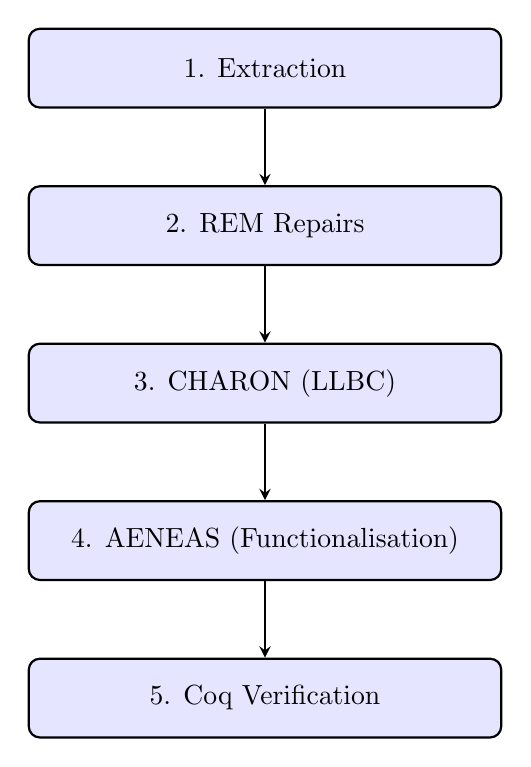
\begin{tikzpicture}[node distance=2cm, >=stealth, thick]
    % Nodes
    \node[draw, rounded corners, fill=blue!10, minimum width=6cm, minimum height=1cm] (extract) {1. Extraction};
    \node[draw, rounded corners, fill=blue!10, minimum width=6cm, minimum height=1cm, below of=extract] (rem) {2. REM Repairs};
    \node[draw, rounded corners, fill=blue!10, minimum width=6cm, minimum height=1cm, below of=rem] (charon) {3. CHARON (LLBC)};
    \node[draw, rounded corners, fill=blue!10, minimum width=6cm, minimum height=1cm, below of=charon] (aeneas) {4. AENEAS (Functionalisation)};
    \node[draw, rounded corners, fill=blue!10, minimum width=6cm, minimum
    height=1cm, below of=aeneas] (coq) {5. Coq Verification};

    % Arrows
    \draw[->] (extract) -- (rem);
    \draw[->] (rem) -- (charon);
    \draw[->] (charon) -- (aeneas);
    \draw[->] (aeneas) -- (coq);
  \end{tikzpicture}
  \caption{Overview of the verification pipeline: from source code extraction to proof of observational equivalence in Coq.}
  \label{fig:verification_pipeline}
\end{wrapfigure}

The verification pipeline augments REM's extract-and-repair workflow with an
automatic equivalence check. Its design is guided by two principles: (1)
verification must require no additional annotations or input from the developer,
and (2) it must complete quickly enough to fit into interactive IDE workflows.
To achieve this, the pipeline translates both the original program $P$ and the
refactored program $P'$ into progressively more structured semantic
representations, culminating in a machine-checked proof of observational
equivalence.

At a high level, the pipeline consists of five stages: \textbf{Extraction},
\textbf{REM repairs}, \textbf{CHARON translation}, \textbf{AENEAS
functionalisation}, and \textbf{Coq verification}. Each stage builds on the
previous one, gradually exposing the semantics of the refactored code while
preserving a clear correspondence to the original. Figure
~\ref{fig:verification_pipeline} provides an overview of the entire process.

\subsection{Extraction}

% Diagrams:
% Either a simple pre an post refactoring code snippet,
% Or a side by side of an example that needs nothing more than copy and paste,
% and a more complex one that needs repairs.

At the first stage, the user identifies a region of code to extract into a new
function. This can be done through REM's CLI, however, the VSCode extension
provides a much more user-friendly interface. The user highlights the code to be
extracted and invokes the extraction command. This step mirrors the mechanics of
traditional Extract Method refactorings: a block is lifted out of its enclosing
function, and a corresponding call is inserted in its place. At this point the
transformation is syntactic and only sometimes results in valid Rust. The below shows both cases:
\begin{itemize}
    \item The first is a simple extraction that requires no further repairs.
    Strict typing makes this a trivial case, and REM would not be called.
    \item The second is a more complex extraction that requires REM's repair
    phase to ensure the refactored code compiles. It is adapted from a real
    commit in \verb|GitOxide|\footnote{\url{https://github.com/GitoxideLabs/gitoxide/commit/c0786717c4979810002365a68d31abbf21d90f2d}},
    and was also used in ``Borrowing Without Sorrowing'' \cite{BorrowingWithoutSorrowing}.
    Note how the extraction algorithm has failed to find the lifetime parameter \verb|'a|, and added an unnecessary borrow of \verb|SectionID|. In this instance, REM would be called to fix the (non-compiling) code.
\end{itemize}

\begin{figure}[h]
\centering
\begin{subfigure}{0.45\linewidth}
  \inputminted[fontsize=\footnotesize, frame=none, linenos=false, breaklines=true, breakanywhere=true]{rust}{3_Chapter3/simple_original.rs}
  \caption{Simple function before extraction}
\end{subfigure}
\hfill
\begin{subfigure}{0.45\linewidth}
  \inputminted[fontsize=\footnotesize, frame=none, linenos=false, breaklines=true, breakanywhere=true]{rust}{3_Chapter3/simple_extracted.rs}
  \caption{Simple function after extraction}
\end{subfigure}

\vspace{1em}

\begin{subfigure}{0.45\linewidth}
  \inputminted[fontsize=\footnotesize, frame=none, linenos=false, breaklines=true, breakanywhere=true]{rust}{3_Chapter3/complex_original.rs}
  \caption{GitOxide function with manual extraction}
\end{subfigure}
\hfill
\begin{subfigure}{0.45\linewidth}
  \inputminted[fontsize=\footnotesize, frame=none, linenos=false, breaklines=true, breakanywhere=true]{rust}{3_Chapter3/complex_extracted.rs}
  \caption{GitOxide function with automated extraction}
\end{subfigure}

\caption{Two extraction examples: a trivial case (top) and a complex, failed case from real-world code (bottom).}
\label{fig:extraction_examples}
\end{figure}



\subsection{REM}

\subsection{CHARON}

\subsection{AENEAS}

\subsection{Coq}
% Potentially include a small paragraph here explaining what Coq is, for the uninitiated.

\section{Proof Obligations}
\label{sec:proof_obligations}

% This section is to be nice and brief. Just a quick overview of the main
% limitations specifically with AENEAS etc. From there, we can point the reader
% to chapter 5 for more details.
\section{Limitations of Current Verification}
\label{sec:limitations_verification}